\chap{Les états (Mode avancé)}\label{ch.states}

Un programme VPL est composé d'une série de paires événement-actions.
\emph{Tous} les événements sont vérifiés périodiquement et les actions appropriées sont effectuées.
Ceci limite les programmes que nous pouvons créer ; pour aller plus loin nous avons besoin d'une façon de spécifier que certaines paires événement-actions sont actives à un certain moment, alors que d'autres ne le sont pas.

Par exemple, quand Thymio devait suivre une ligne (\cref{ch.line}), lorsque le robot sortait de la ligne, nous aurions aimé qu'il tourne à gauche ou à droite afin de rechercher la ligne dans une direction qui dépendait de quel côté il était sorti.
Pour cela, deux paires événement-actions sont nécessaires:
une pour tourner à gauche lorsque le robot sort à droite de la ligne
et une pour tourner à droite lorsqu'il sort à gauche.

%Les états sont disponibles dans le mode \emph{avancé} de VPL.
%Cliquez sur \blksm{advanced} avant de travailler sur les projets de ce chapitre.

\sect{Tape, tape}

Dans les programmes que nous avons réalisé jusqu'ici, nous avons souvent \emph{démarré} Thymio en appuyant sur un de ces boutons et \emph{arrêté} Thymio en appuyant sur un autre.
Mais regardez votre ordinateur, normalement, il n'a qu'un seul bouton pour l'allumer ou l'éteindre.
%\blksm{power-button} 
Le bouton se \emph{rappelle} s'il est dans l'état \bu{allumé} ou l'état \bu{éteint}.

Écrivons un programme qui allume les lumières du robot si vous lui donnez une petite tape et qui les éteigne si vous lui donnez une seconde tape.

{\raggedleft \hfill Programme \bu{tap-on-off.aesl}}

Il est pratique de décrire ce comportement en utilisant un \textit{diagramme d'états} :

\begin{center}
\begin{picture}(240,45)
\thicklines
%\put(0,0){\framebox(240,40){}}
\put(20,20){\circle{40}}
\put(0,0){\makebox(40,40){\textsf{éteint}}}
\put(220,20){\circle{40}}
\put(200,0){\makebox(40,40){\textsf{allumé}}}
\put(40,30){\vector(1,0){160}}
\put(0,30){\makebox(240,10){\textsf{tape $\rightarrow$ allumer}}}
\put(200,10){\vector(-1,0){160}}
\put(0,10){\makebox(240,10){\textsf{tape $\rightarrow$ éteindre}}}
\end{picture}
\end{center}

Ce diagramme comprend deux états indiqués par des cercles, \bu{allumé} et \bu{éteint}.
Depuis l'état \bu{éteint}, le robot peut aller dans l'état \bu{allumé} et revenir, mais seulement en suivant les instructions sur les flèches.
Les instructions décrivent quand une transition d'un état à l'autre peut se produire et comment :

\begin{itemize}

\item \emph{Quand} Thymio est dans l'état \bu{éteint} \textbf{\textit{et}} que l'événement \emph{tape} se produit $\rightarrow$ \emph{allumer} le robot \textbf{\textit{et}} aller dans l'etat \bu{allumé}.

\item \emph{Quand} Thymio est dans l'état \bu{allumé} \textbf{\textit{et}} que l'événement \emph{tape} se produit $\rightarrow$ \emph{éteindre} le robot \textbf{\textit{et}} aller dans l'etat \bu{éteint}.

\end{itemize}

L'accent mis sur le mot \textbf{\textit{et}} avant la flèche~$\rightarrow$ signifie que deux conditions doivent être remplies pour que la transition se fasse: (a) le robot doit être dans un certain état et (b) l'événement doit se produire.
Lorsque les deux conditions sont remplies, alors la transition est prise ce qui fait à la fois changer l'état et exécute l'action écrite après la flèche~$\rightarrow$.

Il est important de réaliser que les deux parties de la condition sont indépendantes.
Dans le diagramme ci-dessus (répété ici),
l'événement \emph{tape} apparaît deux fois, mais l'action 
exécutée lorsque cet événement a lieu 
\emph{dépend de l'état du robot}.

\vspace*{-1ex}

\begin{center}
\begin{picture}(240,40)
\thicklines
%\put(0,0){\framebox(240,40){}}
\put(20,20){\circle{40}}
\put(0,0){\makebox(40,40){\textsf{éteint}}}
\put(220,20){\circle{40}}
\put(200,0){\makebox(40,40){\textsf{allumé}}}
\put(40,30){\vector(1,0){160}}
\put(0,30){\makebox(240,10){\textsf{tape $\rightarrow$ allumer}}}
\put(200,10){\vector(-1,0){160}}
\put(0,10){\makebox(240,10){\textsf{tape $\rightarrow$ éteindre}}}
\end{picture}
\end{center}

\vspace*{-1ex}

Dans un même état, différents événements peuvent causer différentes actions et des transitions vers de nouveaux états différents.
Dans le diagramme suivant, toucher le bouton de gauche
dans l'état \textbf{éteint} allume la lumière verte du robot
et passe l'état du robot à \textbf{allumé1},
alors que toucher le bouton droit \textbf{dans le même état}
entraîne une autre action, allumer la lumière rouge,
et un autre changement d'état vers \textbf{allumé2}.

\vspace*{-1ex}

\begin{center}
\begin{picture}(300,80)
\thicklines
%\put(0,0){\framebox(240,80){}}
\put(25,42){\circle{40}}
\put(10,28){\makebox(30,30){\textsf{éteint}}}
\put(280,20){\circle{40}}
\put(265,6){\makebox(30,30){\textsf{allumé2}}}
\put(40,57){\vector(1,0){220}}
\put(280,65){\circle{40}}
\put(265,50){\makebox(30,30){\textsf{allumé1}}}
\put(40,27){\vector(1,0){220}}
\put(0,60){\makebox(295,10){\textsf{bouton gauche $\rightarrow$ s'allumer en vert}}}
\put(0,30){\makebox(295,10){\textsf{bouton droite $\rightarrow$ s'allumer en rouge}}}
\end{picture}
\end{center}

\sect{Implémenter des diagrammes d'états avec des paires événement-actions}

Nous montrons comment \emph{implémenter} le comportement décrit par le diagramme d'état avec des paires événement-actions.
Implémenter signifie construire un programme qui fera ce que le diagramme d'états ci-dessus décrit.
La \cref{fig.turn-on-off} montre le programme.
Regardons maintenant les paires événement-actions une à une.
Le cercle gauche du bloc \blksm{event-tap-advanced} est
sélectionné (et s'affiche en rouge) pour indiquer qu'il s'agit d'un bloc pour l'événement tape.

\importantbox[Le bloc tape en mode avancé]{
Le bloc pour l'événement tape est différent en mode avancé
car il permet aussi l'utilistation des événements
accéléromètre comme décrit au \cref{ch.angles}.}

\begin{figure}
    \subfigure[Une tape pour allumer la lumière]{
        \label{fig.turn-on-off1}
        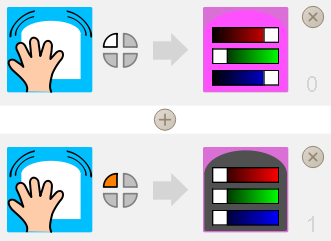
\includegraphics[width=.6\textwidth]{tap-on-off1}
    }
    \subfigure[Une tape pour éteindre la lumière]{
        \label{fig.turn-on-off2}
        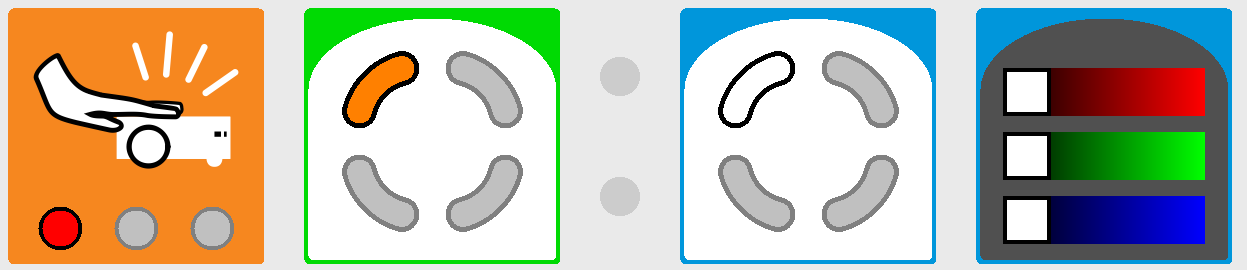
\includegraphics[width=.6\textwidth]{tap-on-off2}
    }
    \caption{Une tape qui a des résultats différents en fonction de l'état.}
    \label{fig.turn-on-off}
\end{figure}

Dans la première paire événement-actions (\cref{fig.turn-on-off1}), l'événement est composé du bloc événement tape avec une indication d'état \blksm{state-filter}.
Un état est indiqué par quatre quartiers d'un cercle, chacun pouvant être soit allumé (orange) ou éteint (blanc).
Dans ce programme, nous utiliserons le quartier en haut à gauche pour indiquer si la lumière du haut du robot est éteinte ou allumée.
Dans \cref{fig.turn-on-off1}, ce quartier est coloré en blanc
et donc la lumière du robot est éteinte.
Ainsi, cette paire veut dire : \textbf{si} le robot est tapé \textbf{et} que le robot est éteint, \textbf{alors} allumer la lumière du robot.

Dans la seconde paire événement-actions
(\cref{fig.turn-on-off2}),
le quartier est coloré en orange et donc la lumière du robot est allumée.
Cette paire veut dire : \textbf{si} le robot est tapé \textbf{et} qu'il est allumé, \textbf{alors} l'éteindre.

Si vous regardez à nouveau le diagramme d'états, vous verrez que seulement la moitié du travail est fait.
En effet, en allumant et éteignant le robot, nous devons aussi changer son état d'\bu{éteint} à \bu{allumé} ou d'\bu{allumé} à \bu{éteint}.
Ainsi, il nous faut ajouter un bloc action \emph{état} \blksm{action-states} à chaque paire.
Ce bloc change l'état selon si les quartiers sont blancs ou oranges.

Pour résumer, la signification du programme de la figure \cref{fig.turn-on-off} est la suivante :

\begin{quote}
    \emph{Quand} le robot est tapé \emph{et} que l'état est \emph{éteint},\\ changer l'état à \bu{allumé} \emph{et} \bu{allumer} la lumière du haut.\\
    \emph{Quand} le robot est tapé \emph{et} que l'état est \bu{allumé},\\changer l'état à \bu{éteint}
    \emph{et} \bu{éteindre} la lumière du haut.
\end{quote}

Chaque événement entraîne à la fois une action lumière et une action état.
Les actions dépendent de l'état dans lequel le robot se trouve, appellé \emph{état actuel}.

\sect{Dans combien d'états différents Thymio peut-il être?}

Quand il est utilisé avec un bloc événement état ou action état, chaque quartier peut être :
\begin{itemize}
	\item \textbf{Blanc}: le quartier est \emph{éteint} ;
	\item \textbf{Orange}: le quartier est \emph{allumé} ;
	\item \textbf{Gris}: le quartier n'est pas pris en compte.
\end{itemize}

Par exemple, dans \blksm{states}, les quartiers en haut à gauche et en bas à droite sont allumés, le quartier en haut à droite est éteint, et le quartier en bas à gauche n'est pas pris en compte.
Ceci veut dire que si \blksmpure{states} est associé à un bloc événement, l'événement se produira si l'état est défini soit par :
\begin{center}
\centering \makebox{\raisebox{-1.7em}{
\includegraphics[height=4em]{states1}}}\quad ou \quad \makebox{\raisebox{-1.7em}{
\includegraphics[height=4em]{states2}}}
\end{center}

Comme chacun des quatre quartiers peut être soit allumé soit éteint, il y a 2 $\times$ 2 $\times$ 2 $\times$ 2 = 16 états :
\begin{quote}
\bu{(éteint, éteint, éteint, éteint)\\(éteint, éteint, éteint, allumé)\\(éteint, éteint, allumé, éteint)\\
\mbox{}\hspace{3em}\ldots\\
(allumé, allumé, allumé, éteint)\\
(allumé, allumé, allumé, allumé)}.
\end{quote}
La \cref{fig.all-states} montre tous les états possibles.
\importantbox{L'état courant du robot est toujours affiché sur le haut du robot par les quatre arcs de cercles lumineux.
Par exemple, la \cref{fig.state-leds} montre le robot dans l'état \bu{(allumé, allumé, allumé, allumé)}.}

\trickbox[Information]{Lorsqu'un programme démarre, l'état initial est toujours 
\bu{(éteint, éteint, éteint, éteint)}:\quad \blkmed{state-all-off}}

\trickbox{Si vous n'utilisez pas tous les 16 états possibles, mais par exemple que 2 ou 4, vous êtes libre de décider quel quartier vous utiliser pour représenter votre état.
Aussi, si par exemple vous avez deux choses différentes à encoder dans l'état, et que chacune d'elle a deux valeurs possibles, vous pouvez utiliser deux quartiers indépendemment.
C'est pourquoi la capacité d'\emph{ignorer} un quartier est très utile !
Essayez toujours de rester le plus simple possible.
}

\begin{figure}
	\subfigure[Tous les états possibles de Thymio]{
		\label{fig.all-states}
		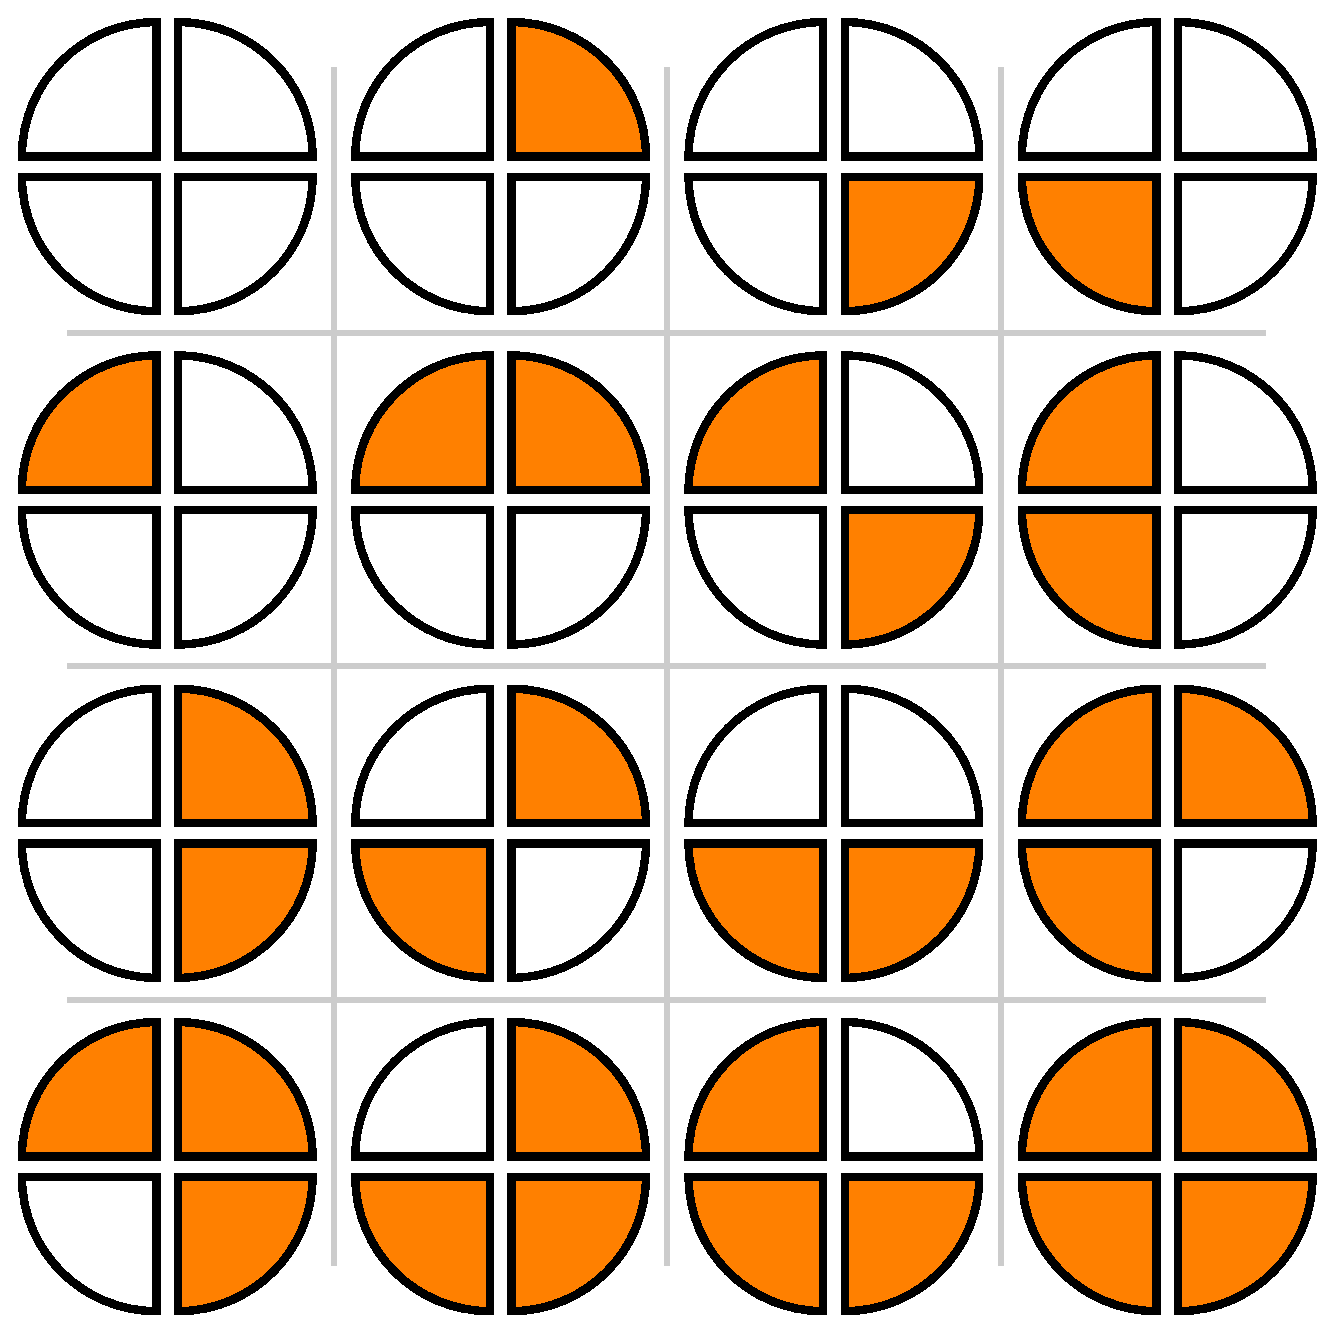
\includegraphics[width = 0.4\textwidth]{all-states}
	} 
	\hfill
        \subfigure[La cercle de lumières indique l'état]{
		\label{fig.state-leds}
		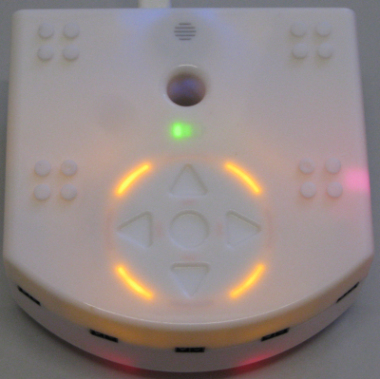
\includegraphics[width = 0.4\textwidth]{state-leds}
	}
	\caption{Les états de Thymio et leur représentation}
\end{figure}

\sect{Attraper la souris}

Écrivons un programme qui fasse tourner le robot de droite à gauche à la recherche d'une souris (ou d'un autre objet).
Si le robot détecte une souris avec son capteur tout à gauche, il continue la recherche jusqu'à ce que la souris soit détectée avec son capteur tout à droite.
Puis, il se positionne en face de la souris, comme sur la \cref{fig.cat-mouse}.

{\raggedleft \hfill Programme: \bu{mouse.aesl}}

Le diagramme d'état suivant décrit le comportement du robot:

\begin{center}
\unitlength=1.2pt
\begin{picture}(320,35)
    %\put(0,0){\framebox(320,35){}}
    \put(40,10){\oval(80,20)}
    \put(160,10){\oval(80,20)}
    \put(280,10){\oval(80,20)}
    \put(0,0){\makebox(80,20){\bu{chercher à gauche}}}
    \put(120,0){\makebox(80,20){\bu{chercher à droite}}}
    \put(240,0){\makebox(80,20){\bu{trouvé}}}
    \put( 80,10){\vector(1,0){40}}
    \put(200,10){\vector(1,0){40}}
    \put(40,35){\vector(0,-1){15}}
\end{picture}
\end{center}

\begin{enumerate}
\item Lorsque le bouton central est touché, le robot entre dans l'état \bu{chercher à gauche} et 
    tourne de droite à gauche.
\item Lorsque le robot est dans l'état \bu{chercher à gauche}
    et détecte la souris sur son capteur tout à droite,
    il prend l'état \bu{chercher à droite} et tourne de gauche à droite.
\item Lorsque le robot est dans l'état \bu{chercher à droite}
    et il détecte la souris avec son capteur central,
    il prend l'état \bu{trouvé} et s'arrête.
\end{enumerate}

L'essentiel est de remarquer que lorsque le capteur central détecte la souris,
le robot s'arrête \emph{seulement si} le robot est dans l'état \bu{chercher à droite}.
Sinon (si la souris est détectée par le capteur central en mode \bu{chercher à gauche}), rien ne se produit.

\begin{figure}
    \begin{center}
        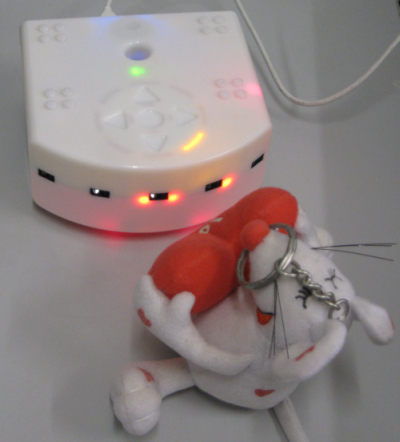
\includegraphics[width=0.4\textwidth]{cat-mouse}
	\caption{Le robot chat cherche la souris}
        \label{fig.cat-mouse}
    \end{center}
\end{figure}

Implémentons ce comportement.
L'état du robot sera défini par le quartier supérieur gauche.
Choisissons le blanc pour représenter l'état \bu{chercher à gauche} et l'orange pour représenter l'état \bu{chercher à droite}.
Puisque le programme se termine lorsque la souris est détectée dans l'état \bu{chercher à droite},
nous n'avons pas besoin de représenter l'état final \bu{trouvé}.
Initialement, tous les quartiers sont \bu{éteints} (blancs).

La paire événement-actions suivante fait tourner le robot à gauche : \blkc{mouse1}
Quand le bouton central est touché, l'état change et devient
\bu{chercher à gauche} \emph{et} le robot tourne à gauche.

%Ceci se produira lorsque le quartier gauche-haut est éteint ; initialement tous les quartiers de l'état sont éteint.

La prochaine paire événement-actions implémente la deuxième étape: \blkc{mouse2}
Quand le robot est dans l'état \bu{chercher à gauche} et
que la souris est détectée par le capteur tout à droite,
l'état devient \bu{chercher à droite}
\emph{et} le robot tourne vers la droite.

Notez que le petit carré à côté de ce capteur est noir pour que l'événement se produise seulement si seul le capteur le plus à droite détecte la souris.

La troisième étape est implémentée dans la paire événement-actions suivante: \blkc{mouse3}
Lorsque la souris est détectée par le capteur central dans l'état \bu{chercher à droite}, le robot s'arrête.


%Pourquoi l'événement de cette paire doit-il dépendre de l'état ?
%La raison est que le capteur central détectera aussi la souris durant le scan initial de droite à gauche.
%Nous voulons que le robot fasse d'abord un scan complet avant de retourner à la position de la souris ; il est donc nécessaire que cette première détection soit ignorée.
%Ceci est accomplit en arrêtant le scan seulement lorsque l'état est \bu{allumé} et ceci arrive que lorsqu'un scan complet a été effectué.

\trickbox{
Il vous faudra expérimenter avec la distance de la souris au robot.
Si elle est trop proche du robot, les capteurs à côte du capteur central détecteront aussi la souris, alors que l'événement demande qu'ils ne la détecte \emph{pas}.
}

\bigskip

\bigskip

\exercisebox{\thechapter.1}{
Écrivez un programme qui fasse danser le robot : il tourne à gauche sur place durant deux secondes, puis tourne à droite sur place durant trois secondes.
Ces mouvement se répètent indéfiniment.
}

\bigskip

\exercisebox{\thechapter.2 (Difficile)}{
Modifier le programme de suivi de ligne du \cref{ch.line} pour que le robot tourne à gauche quand il sort de la ligne par le côté droite, et qu'il tourne à droite quand il sort de la ligne par le côté gauche.
}
